\documentclass[letterpaper,english,prl,reprint,longbibliography]{revtex4-1} %twocolumn,

%\usepackage[latin9]{inputenc}
\setcounter{secnumdepth}{3}
\usepackage{babel}
\usepackage{amsmath}
\usepackage{amssymb}
\usepackage{graphicx} 
\usepackage{epstopdf} %add for pdflatex, nut don't compile because of invisible character copied from .bbl file?
\usepackage[T1]{fontenc}
\usepackage[utf8x]{inputenc} 
\usepackage{esint}
\usepackage{verbatim}
%\usepackage[hyphens]{url}
\usepackage[unicode=true]{hyperref}
\usepackage[table]{xcolor}
\newcommand{\re}[1]{\textcolor{red}{#1}}
%\loadpackage{url}
%\usepackage[unicode=true]{hyperref}
%\setcounter{biburllcpenalty}{7000}
%\setcounter{biburlucpenalty}{8000}
%\usepackage{breakurl}
%\hypersetup{breaklinks=true}
%\usepackage[hyperref,eprint=false]{biblatex}
\makeatletter

%%%%%%%%%%%%%%%%%%%%%%%%%%%%%% LyX specific LaTeX commands.
\pdfpageheight\paperheight
\pdfpagewidth\paperwidth

%%%%%%%%%%%%%%%%%%%%%%%%%%%%%% User specified LaTeX commands.
\usepackage{bbold}
\newcommand{\overbar}[1]{\mkern 1.5mu\overline{\mkern-1.5mu#1\mkern-1.5mu}\mkern 1.5mu}
\usepackage{xcolor}
\hypersetup{
    colorlinks,
    linkcolor={red!50!black},
    citecolor={blue!50!black},
    urlcolor={blue!80!black}
}

\makeatother

\begin{document}

\preprint{APS/123-QED}

\title{Inferring repertoire dynamics from repertoire sequencing}

\author{Maximilian Puelma Touzel}
%\email[]{puelma@lpt.ens.fr}

\affiliation{Laboratoire de Physique Théorique, ENS-PSL Research University, Paris, France}

\author{Aleksandra Walczak}

\affiliation{Laboratoire de Physique Théorique, ENS-PSL Research University, Paris, France}

\author{Thierry Mora}

\affiliation{Laboratoire de Physique Statistique, ENS-PSL Research University, Paris, France,}

\vspace{0.5cm}

\begin{abstract}
High-throughput sequencing provides access to expression-level detail of cell populations. Identifying signal in this data is nevertheless a challenge: intrinsic variability, vast sub-sampling, and indirect access together make difficult the reliable and accurate inference of the changes in population size due to environmental perturbations. Here, in the context of antigen-perturbed immune cell repertoires, we formulate access to the unobserved repertoire using a generative model of observed sequence count pairs from a reference and differentially-expressed condition. When applied to pairs of replicates, our model captures the natural variability in the system, giving reproducible behavior across donors and, in spite of sup-sampling, provides plausible parameter estimates for the unobserved repertoire. Using this replicate model as a baseline, we then formulate the differentially expressed condition using a prior distribution of the ratio of a clone’s frequency pair for pairs of repertoires sampled at different time points. The posterior distribution of this ratio for each observed clone is then obtained and used to characterize if and how it participates in the response. Applying our approach to yellow fever vaccination as a model of acute infection in humans, we identify candidate clones participating in the response.   

\end{abstract}

\keywords{keywords}

\pacs{}

\maketitle
%\section{Introduction}
\begin{itemize}
%\item Power-law clone size distributions are observed for sequenced uncompartmentalized repertoires. Various candidate mechanisms underlying power law (mixture of birth death etc. ref. desponds). Nevertheless, what is clear is that simple birth death alone is excluded since it gives exponential distribution that has no long, power law tail.
\item background: Next generation sequencing gives access to repertoire wide data containing information that can inform more comprehensive analysis repertoires and more robust vaccine design;
\item Problem: quantification of repertoire response dynamics:
\item To ongoing, natural stimuli, modelled as a point process of infections, giving rise to diffusion-like response dynamics. Or
\item to a single, strong perturbation, such as a vaccine, giving rise to a stereotyped, transient response dynamics
\item Conventional approaches
\begin{itemize}
	\item DESEQ2
	\item Edge R
\end{itemize}
\item  Their limitations
\item  Our approach...
\end{itemize}

% Background:

% Frontline ADAPTIVE immune system. $~10^{11}$ cells. $\leq 10^8$ clones. not directly observable .intrinsically variable/fluctuating
% selected repertoire sculpted by infection and vaccination history
% Its approximately $10^{11}$ lymphocytes that make up at least $10^8$ number of clones, the cells in each clone express the same receptor. 
% We don’t access the full repertoire, but only observe a small subsample of it. 
% The full repertoire and thus our samples of it vary across individuals, and even from replicates within the same individual. 
% It is also sculpted by infection and vaccination history so ...
% If we sample in time we see changes to the repertoire, and in particular as they respond to an intervening perturbation, like a vaccine. 

Final Paragraph:

Here, we first quantify the natural variation (either same-day replicate or different day non-perturbation containing) in a learned generative model of receptor RNA count-pair statistics. Next, we then construct a differential expression model by augmenting this null model with the hidden log fold-change of clone frequency between the two compared conditions, learning a prior on such change from the data. Seeing how the parameters of this prior vary across time-point comparisons provides the repertoire dynamics at ensemble-level of description. Finally, we show how our learned model can be used to infer a posterior probability distribution of fold change for any observed count pair, and thus any specific clone, that can be used to infer the temporal changes of that clone's frequency. The structure of the contribution of singleton clones, the vast majority of all clones in the sample, reflect the balance between of the power of the power-law form of clone frequency density preferencing near maximal expansion and our conservative choice of prior preferencing expansion of a characteristic size. The uncertainty in the inferred expansion obtained from these posteriors is over-dispersed, roughly uniform over the range of expansion for singleton clones appearing in the differentially expressed condition.  As an example, we use the posterior expansion probability to generate a list of clones significantly expanded by YF vaccination. 

\section*{Model family}
We consider a family of generative models of pair count statistics of observed immune receptor RNA molecules obtained by sequencing blood samples taken in a reference and test pair of conditions, respectively. 
For our purpose, an immune repertoire is a finite set of $N$ clones with frequencies $\vec{f}=(f_1,\dots,f_N)$, over the domain $f_i\in[f_{\textrm{min}},1]$, where $f_{\textrm{min}}$ is the minimum allowed frequency of corresponding to a single lymphocyte. A prior density over clone frequencies is given by $\rho(f)$. $N$ and $f_{\textrm{min}}$ must be determined self-consistently when defining the corresponding joint density, 
\begin{eqnarray}
	\rho_N(\vec{f})\propto \prod_{i=1}^N\rho(f_i)\delta(Z_f-1)\;,\label{eq:jointf}
\end{eqnarray}
where the Dirac delta-function, $\delta(x)$, is used to impose a normalization constraint on the sum of frequencies, $Z_f=\sum_{i=1}^N f_i$, 
\begin{align}
  Z_f=1\;. \label{eq:norm_constr}
\end{align}

Each clone's frequency pair from the reference and test conditions impacts its chance of being picked up in a realization of the acquisition process consisting of pair sampling and sequencing. 
We present a model, $P(n,n',f,f')$, based on the priors $\rho(f)$ and $\rho(f')$, with $f$ and $f'$ and $n$ and $n'$ denoting a clone's frequencies and receptor molecule counts in the reference and test condition, respectively. In general, repertoires are dominated in number by small clones missed in the acquisition process. Thus, in any realization, $n+n'>0$ for only a relatively small number, $N_{\textrm{\textrm{obs}}}\ll N$, of clones, which can still be large since $N$ is typically $ 10^6$ ($10^9$) for mouse (human). These \emph{observed} clones are those captured in the blood sample and amplified above detection levels in the sequencer in at least one of the test and reference conditions. We have no experimental access to the \emph{unobserved} clones that realize with $n+n'=0$. Marginalizing over $f$ and $f'$ and conditioning on $n+n'>0$, we obtain the model prediction for what we observe, 
\begin{align}
	P(n,n'|n+n'>0)=\frac{1-\delta_{n0}\delta_{n'0}}{1-P(0,0)}P(n,n')\;,
\end{align} 
i.e. the distribution of pair counts from observed clones. The model estimate for the total number of clones is then $N=N_{\textrm{\textrm{obs}}}/(1-P(0,0))$. 
%These are the union of two sets of \emph{observed} clones, i.e. clones that are captured in the blood sample and amplified in the sequencer in either of the two conditions, providing a finite number of molecules in at least one of the reference-test pair.
%The unobserved frequencies of these observed clones directly impact the model's observed distribution, $P(n,n')$, of molecule count pairs, $n$ and $n'$, in the reference and test condition, respectively (Fig.\ref{fig:nullstats}A; see Methods section for details). 

The $N-N_{\textrm{\textrm{obs}}}$ \emph{unobserved} clones influence the count statistics only via the presence of their frequencies in the two normalization constraints, $Z_f=1$ and $Z_{f'}=1$, so far unaccounted for in the model.
In the Methods, we show that $Z_f=1$ is implicitly satisfied if 
\begin{equation}
	N\langle f\rangle=1\;,\label{eq:orignorm}
\end{equation}
which also imposes the desired self-consistency between $f_\textrm{min}$ and $N$. We employ this constraint in our clone model. Equivalently, it is expressed using the frequency posteriors, which we separate into unobserved and observed contributions,
\begin{align*}
	%1&=\langle Z\rangle_{\prod_i^N\rho(f_i|\mathcal{D})}\\
	%&=\sum_i^N \langle f_i\rangle_{\rho(f_i|\mathcal{D})}\\
	1&= NP(0,0) \langle f\rangle_{\rho(f|n+n'=0)}+	N\sum_{n+n'>0}P(n,n')\langle f\rangle_{\rho(f|n,n')}\;.
\end{align*}

$Z_f$ and $Z_{f'}$ are insensitive to the precise values of a realized set of unobserved clones, and their average frequency is well approximated as the ensemble average in first term above. In contrast, the sum of frequencies of the observed clones might depend on the realization, especially in the case of large, outlying clones arising from power-law distributed clone sizes. This sensitivity can nevertheless be incorporated into the model by using the approximation $\sum_{n+n'>0}P(n,n')\approx \frac{1}{N}\sum_{i=1}^{N_\textrm{obs}}$ so that the second term is $\sum_{i=1}^{N_{\textrm{obs}}}\langle f\rangle_{\rho(f|n_i,n'_i)}$. We define the right-hand side of this realization-dependent constraint 
\begin{align}
	%1&=\langle Z\rangle_{\prod_i^N\rho(f_i|\mathcal{D})}\\
	%&=\sum_i^N \langle f_i\rangle_{\rho(f_i|\mathcal{D})}\\
	Z^\mathcal{D}_f&= N	P(0,0)\langle f\rangle_{\rho(f|n+n'=0)} + \sum_{i=1}^{N_{\textrm{obs}}}\langle f\rangle_{\rho(f|n_i,n'_i)}\;.\label{eq:postnorm}
\end{align}
and impose that $Z^\mathcal{D}_f=1$, in addition to $N\langle f\rangle=1$. We note that while not equivalent, differences in values of parameters learned with each constraint separately were small, suggesting there is a high overlap in the respective regions of the parameter space satisfying the original  \ref{eq:orignorm} and realization-dependent \ref{eq:postnorm} constraints (Supp.Fig.X). We impose an equivalent constraint for $\vec{f}'$, via the equivalent condition, 
\begin{align}
	Z^\mathcal{D}_{f'}=Z^\mathcal{D}_f\;.\label{eq:fprimeconst}
\end{align}

% Sampling from the models would be more aligned with the inference if $N_{\textrm{obs}}$ was a parameter. In that case, we need only sample the observable clones.
%$\langle Z \rangle_{\rho(\vec{f})}}$
%As a result the joint frequency factorizes and $\langle Z\rangle_{\rho(f)}\approx N\langle f\rangle_{\rho(f)}$ (same for $Z'$).
%Thus, in addition to these two constraints, choosing $N$, and the parameters of $\rho(f)$, and $\rho(f')$ to be mutually consistent demands the constraint that $N\langle f\rangle_{\rho(f)}=1$ and $ N\langle f'\rangle_{\rho(f')}=1$, respectively (the latter can be equivalently expressed as $\langle f'\rangle_{\rho(f')}=\langle f\rangle_{\rho(f)}$). For arbitrary test condition, the latter average isn't necessarily defined. implies that $Z$ and $Z'$ are near unity. When sampling differential expression models, we must also normalize $f'$ by $Z'$.
%As a result, 
%When inferring models, we impose the constraint $N\langle f\rangle_{\rho(f)}=1$ the same normalization, but conditioned on the observed data 
%\begin{equation}
%	1=N\langle f\rangle_{\rho(f|\mathcal{D})}
%							   = P(0,0)N\langle f\rangle_{\rho(f|n+n'=0)} + \sum_{i}^{N_{\textrm{obs}}}\langle f\rangle_{\rho(f|n_i,n'_i)}\;.
%\end{equation}
%and similarly for $f'$. Does this reduce to $N\langle f\rangle_{\rho(f)}=1$?

%sampling section:
%Sampling from the models would be more aligned with the inference if $N_{\textrm{obs}}$ was a parameter. In that case, we need only sample the observable clones.
%For differential expression models With $N$ a fixed input parameter to the sampling procedure, sampled frequencies are simply normalized by dividing by $Z$. For the differential expression model, we in addition impose that $\langle f\rangle=\langle f'\rangle$.


%In this case, the normalization when sampling from the model is implementation of the normalization depends on whether sampling from or inferring the parameters of the model, and also whether we are considering the null or differential expression model.
%We present each form of the normalization used in its respective section.

Finally, we take the `common dispersion' approach \citep{Robinson2008}, in which we assume that $n$ and $n'$ are conditionally independent once the reference and test frequency are given, and that their statistics depend only implicitly on clone identity (\emph{i.e.} clonal sequence) via these frequencies.
Defined models were fit using a pair count dataset, $\mathcal{D}=\{(n_i,n'_i)\}_{i=1}^{N_{\textrm{\textrm{obs}}}}$, by maximizing the $\log$ marginal likelihood of the data, $\sum_{i=1}^{N_{\textrm{\textrm{obs}}}} \log P(n_i,n'_i|\theta)$, over the free parameters, $\theta$, subject to the above constraints.
%See Appendix for the derivation of this single clone model from the full density over the entire repertoire of all clones. \textcolor{red}{(include this?)}. 

Our method to determine differential expression proceeds in two steps, where in each we define, learn, and analyze an instance of this model family.
In the first step, we consider a null model in which a replicate, e.g. same-day sample, is given for the test condition. 
In this case, the reference and test frequency are the same and no additional constraint for $\vec{f'}$ is needed.
The learned parameters of $\rho(f)$ and the acquisition model from this pair serves to define the baseline, e.g. pre-vaccination statistics.
In the second step, we consider a model for differential expression in which a differentially expressed condition serves as the test, e.g. the reference and test condition being pre- and post-vaccination, respectively. 
The parameters of $\rho(f)$ and the acquisition model here are set to those of the null model. 
As a result, $Z^\mathcal{D}_f$ is not unity, but in practice we find it is close, and thus so is $Z^\mathcal{D}_{f'}$ on account of the constraint on $\vec{f'}$, eq.\ref{eq:fprimeconst}.  
What is different here is $\rho(f')$: the test frequency, $f'$, is obtained from a transformation of the reference frequency, $f$.  
This transformation summarizes the effect of the dynamics assumed to act on clone sizes during the time period between the two samples. 
In the absence of a strong perturbation such as a vaccine or acute infection, this dynamics is dominated by the diffusive behavior of some stochastic population dynamics for which the transformation is given by the corresponding Green's function.  
For a strong, transient perturbation, in contrast, time-translation invariance is broken and a transformation tailored to the properties of the transient perturbation must be specified. 
In the context of immune response to yellow fever vaccination, we focus on the latter. 
%Throughout, the optimization was performed subject to the normalization constraint, $\langle \sum_i^N f_i\rangle=1$, where $N$ is the (unobserved) total number of clones in the repertoire and angle brackets denote ensemble average. 
%Bringing the average into the sum gives $N\langle f \rangle=1$, approximately satisfied for $N$ large enough that the approximation $\langle f \rangle \approx \frac{1}{N}\sum_i^{N}f_i$ becomes valid on account of the law of large numbers. 
%The latter applies here since we define $f$ over the closed interval $\left[f_{\textrm{min}},1\right]$ so that the ensemble average $\langle f \rangle=\int f\rho(f)\textrm{d}f$ always exists, even for the power law form of $\rho(f)$, which we choose throughout.
%The resulting constraint, $\langle f \rangle=(1-P(0,0))/N_{\textrm{\textrm{obs}}}$ was enforced at each step of the learning and can be viewed as restricting the family of considered models to those for which the joint density of clone frequencies factorizes. {\color{red}More here on $\vec{f}$?}.

\section*{Results}
\subsection*{A null model for replicate clone size variation}
Using this model family, we defined a null model of count statistics and fit it to a pair of replicates, here defined as coming from the same blood sample. 
This model provides a baseline variability with which differential expression can after be assessed. 
The marginal pair count distribution of this null model is  
\begin{eqnarray}
	P(n,n'|\theta_{\textrm{null}})=\int P(n|f)P(n'|f'=f)\rho(f)\text{d}f\;,
\end{eqnarray}
where we have collected the parameters into $\theta_{\textrm{null}}$. 
The influence of $f$ on $P(n|f)$ is an explicit parametrization, e.g. where $P(n|f)$ is a Poisson distribution with mean proportional to $f$ (see Fig.\ref{fig:nullstats}B). 
Current methods, e.g. \cite{Robinson2008}, more accurately model $P(n|f)$ by accounting for its observed over-dispersion using a negative binomial distribution. 
The number of cells of a clone in the sample, $m$, is an additional random variable in the measurement process chain, which has so far been neglected. 
Thus, in a further refined choice for $P(n|f)$, we explicitly account for this step by choosing $P(m|f)$ as a negative binomial distribution and then $P(n|m)$ as a Poisson distribution, giving $P(n|f)=\sum_m P(n|m)P(m|f)$. 
This two-step model, as a more explicit representation, more accurately captures the count statistics of the measurement process, especially at low counts. 
The latter fact arises from the power-law nature of frequency distribution, for which the frequency of most clones falls below the sampling depth so that the majority of clones are not captured in the sample. 
These low frequency clones are so numerous, however, that the sample is nevertheless dominated by them, each appearing at the minimum finite size. 
For a single-step model, the minimal size of a clone is a single molecule. 
For a two-step model, in contrast, the minimal clone size is a single cell, which gives a small, but variable number of molecules. 
The one and two-step models thus leave different signatures at low counts, even for the additional dilution of counts due to PCR inefficiency during the sequencing of the sample \citep{Best2015a}.
We find that, indeed, this two-step model exhibits a better fit to data (see Fig.\ref{fig:nullstats}B; Supp fig\textcolor{red}{(suppmat figure from misha paper)}), especially for clones captured with few counts (see Supp. Fig. 1). 
The fit for the over-dispersed, one-step model is not significantly worse however, while the one-step Poisson model is clearly a poor choice, as it fails to capture the over-dispersion.

\begin{figure}[ht!]
% \includegraphics[width=\linewidth]{fig1_nullmodel}
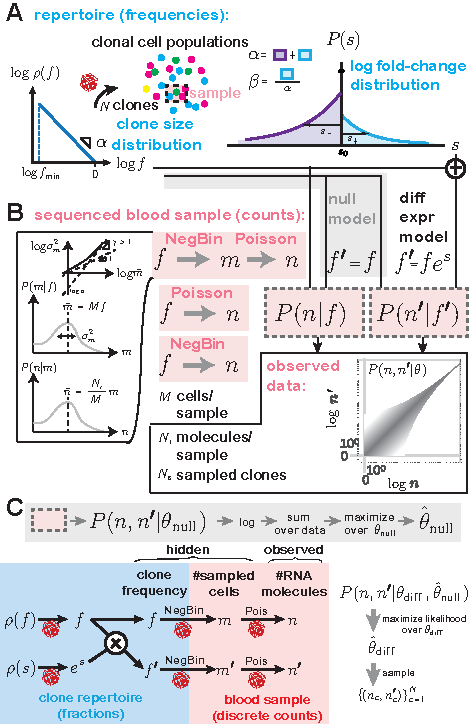
\includegraphics{fig1_nullmodel_v3}
\centering{}
\caption{
\emph{Repertoire model}. 
(a) Clone frequency distribution, $\rho(f)$, is set as a power law, parameterized by the power, $\alpha$ and the minimum frequency, $f_{min}$.
(b)
(c) Differential expression model structure and learning procedure. Null model parameters are learned by marginalizing over clone frequency, $f$, and maximizing this marginal likelihood with respect to the parameters. Sampled repertoires can then be generated using the ML estimate. $P(n|f)$ is set as a negative binomial distribution in cell counts controlling the scale parameter of a Poisson distribution of molecule counts. In the differentially expressed condition (prime-decorated quantities), the parameters, $\theta_{diff}$, of the prior distribution, $\rho(c)$, of fold-change, $c$, are learned by maximizing the marginal likelihood (see section \textit{Fold change prior}) with respect to $\theta_{diff}$, keeping the remaining parameters, $\theta_{null}$, fixed to their ML estimates, $\hat{\theta}_{null}$, previously obtained using same-day replicate data (see fig. \ref{fig:nullstats}).
\label{fig:fullmodel}}
\end{figure}

\begin{figure}[ht!]
% \includegraphics[width=\linewidth]{fig1_nullmodel}
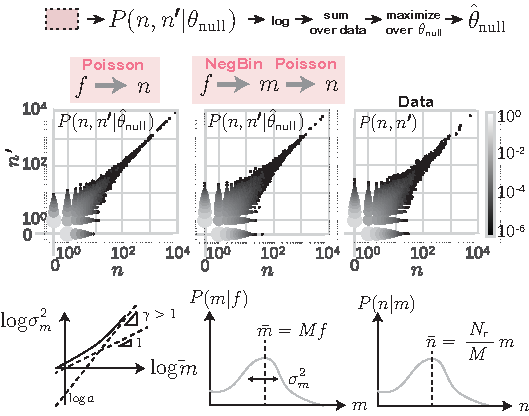
\includegraphics{fig1_nullmodel_v5}
\centering{}
\caption{
\emph{Learning a null model}.  Models and data comparison using molecule pair count statistics (example donor: S2; day 0-day 0 comparison). The learned model for Poisson distributed $P(n|f)$ (left) and for $P(n|f)$ set as a negative binomial distribution in cell counts controlling the scale parameter of a Poisson distribution of molecule counts (center; fig.\ref{fig:modelstruct}). Right: empirical pair count histogram.  
\label{fig:nullstats}}
\end{figure}

\begin{figure}[ht!]
%\includegraphics[width=\linewidth]{fig2_learnednullparas}
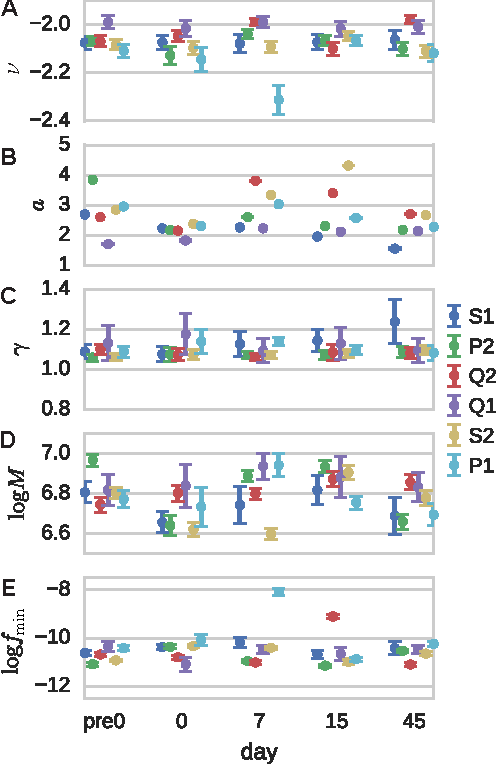
\includegraphics{fig3_learnednullparas}
\centering{}
\caption{
\emph{Learned null model parameters} plotted separately for each donor and time point. Error bars are the inverse standard deviation of a Gaussian approximation around the maximum of the likelihood acting as a lower bound for the variance of the estimates. 
\label{fig:nullparas_timeseries}}
\end{figure}

\begin{figure}[ht!]
\includegraphics[width=\linewidth]{conditional_marginal}
\centering{}
\caption{
\emph{Null model marginals and conditionals}. The marginal, $P(n_1|\theta_n)=\sum_{n_2}P(n_1,n_2|\theta_n)$ (a), and conditional $P(n_1|n_2\theta_n)=P(n_1,n_2|\theta_n)/P(n_1|\theta_n)$ (b), distributions.{\color{red} Add conditional $P(n|n'=0)$ and $P(n'|n=0)$. clean up figure (remove grey etc.)}
\label{fig:modelfit}}
\end{figure}

\begin{figure}[ht!]
%\includegraphics[width=\linewidth]{fig2_learnednullparas}
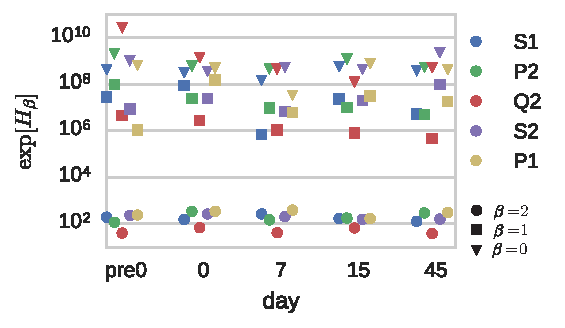
\includegraphics{fig4_div_estimates}
\centering{}
\caption{
\emph{Diversity estimates.} Shown are diversity estimates obtained from the Renyi entropies, $H_\beta$, of the inferred clone frequency distributions for $\beta=0$ (estimated total number of clones, $N$), $\beta=1$ (Shannon entropy) and $\beta=2$ (Simpson index), across donors and days.
\label{fig:div_estimates}}
\end{figure}

% \begin{figure*}[ht!]
% \includegraphics[width=\textwidth]{fig2_learnednullparas}
% \centering{}
% \caption{
% \emph{Histograms of learned null model parameters}. The clone frequency distribution $\rho(f)=\int_{f_{min}}^{1}f^\alpha\textrm{d}f/Z$, is determined by the power $\alpha$ and minimal frequency, $f_{min}$. The cell count variance, $\sigma^2_m=fM+a(fM)^\gamma$, is determined by the total number of cells in the sample, $M$, and the power, $\gamma$, and coefficient, $a$, controlling the over-dispersion.{\color{red}update figure with remaining data}
% \label{fig:nullparas}}
% \end{figure*}

% Here we provide an accurate, process-based model of the observed variability of RNA count pairs obtained from pairs of same-day replicates sampled together, but sequenced separately (see Fig. \ref{fig:nullstats}).
% %We developed four process-motivated generative models for the replicate count-pair distribution (see table \ref{Tbl1:NullModelCompare} and Fig.\ref{fig:modelstruct}). 
% Our model maps clone frequency to observed number of RNA receptor molecules, via the number of cells of that clone captured in the sample (see fig.\ref{fig:proc}). This two-step process better captures the behaviour of the clones captured with few counts (see Supp. Fig. 1). Presumably, this is because the smallest clone size in the sample is a single cell, which gives a variable number of RNA receptor molecules, whereas a single step process of RNA counts alone would give just a single count. 

The null models were fit by maximizing the $\log$ marginal likelihood of the data, $\sum_{i=1}^{N_{\textrm{\textrm{obs}}}} \log P(n_i,n'_i|\theta_{\text{null}})$, over the parameters, $\theta_{\text{null}}$. 
For the two-step model, the parameters are $\theta_{\text{null}}=(\alpha,M,a,\gamma,f_{\textrm{min}})$, where $\alpha$ is the power law exponent, $M$ is the total number of cells, $a$ and $\gamma$ are the coefficient and power of the over-dispersion term in the mean variance relation of the negative binomial distribution of cells, and finally, $f_{\textrm{min}}$ is the minimum allowed clone frequency.
We developed a sampling protocol for this model (see Methods) and used it to validate our inference algorithm (Fig. \ref{fig:reinfer_null}). Next, we assessed the ability of the two-step model to capture the observed count pair statistics obtained from the same-day replicates, across days and donors. 
Figure \ref{fig:nullparas_timeseries} shows the learned values for 30 null models calculated from same-day replicates from 6 donors sampled over 5 time points spanning a 1.5 month period. 
The variability across donors and days is \textcolor{red}{... indicating a degree of regularity to the natural variability.} 
The learned values of $M$ are consistent with rough estimates obtained from the known sample volume (personal communication, M. Pogorelyy), and the reciprocal of the learned values of $f_{\textrm{min}}$ give plausible estimates for the total number of lymphocytes in the body.
The uncertainty associated with these estimates was assessed using the lower-bound provided by the curvature of the likelihood function around the optimum, \emph{i.e.} the Fisher information, of the optimization problem without the normalization constraint. 

We confirmed that the learned values of the parameters provide a good fit to the pair count statistics via the model's prediction of the conditional and marginal distributions of pair counts, whose correspondence with their empirical counterparts is not required by the fitting procedure (see Fig.\ref{fig:modelfit}). For example, Fig. \ref{fig:modelfit}A shows that marginal, $P(n)$, inherits the power law of the clone frequency distribution, but exhibits deviations from this law at low count number consistent with the data and the prevalence of clones in the sample with putative frequencies less than $1/N_{\textrm{\textrm{obs}}}$. We also note that the model does well at capturing the count statistics in one condition when there are no observed counts in the other condition \textcolor{red}{(need to add this plot)}.

The learned models provide a clone frequency distribution, $\rho(f)$, that, together with the observed number of clones in one sample can be used to estimate measures of diversity of the repertoire producing that sample (see Methods). In Fig. \ref{fig:div_estimates}, we show the values, across donor and days, of the $\beta=0,1,2$ Hill diversities as three distinct diversity metrics: the species richness, i.e. the total number of clones; the Shannon diversity as the effective number of clones obtained from a uniform distribution of their frequencies; and the Simpson diversity, the expected number of shared clones between two realized repertoires. \textcolor{red}{Discuss the variability here?} We note that diversity estimates obtained from observed species abundance are affected by statistical bias \citep{Mora2016}.

\textcolor{red}{Paragraph on control result showing negligible diffusive effect (develop and include, or leave out?):}

Both the intrinsic and driven fluctuations of the population dynamics of immune receptor repertoires imply that clone frequencies will vary across days, even in the absence of any antigen-driven response. 
If the timescale of this diffusive effect falls within the transient response time, the variability of pair count statistics over this window will be structured by both types of fluctuations. 
in such a short time window, however, we cannot infer the diffusive component reliably, and we omit this component.
Fitting the presented model, which lacks an explicit diffusive component, in the window might inaccurately attribute differential expression to what is actually natural clone size dynamics. 
However, in the case of our yellow fever dataset, we can learn a pair of null models, each for two time points separated by the same length of time just before and after vaccination, respectively, and compare the variability of each to that of the null model previously learned from same-day replicates (see fig. X). 
While we find that indeed the null model obtained from separated time points has higher variability, it is significantly lower than the variability of null models learned for pairs of time points with greater time separation. 
This suggests that our inference of differential expression discussed in the next section is unbiased by the diffusive contribution to the population dynamics. 

% \begin{itemize}
% 	\item  presentation question: do we start with data description and plot first (See figure above) or immediately develop model first and only show data when showing fit?
% \end{itemize}

% \begin{table*}%[H] add [H] placement to break table across pages
% \caption{Null Model Selection. Akaike Information Criterion (AIC) and Bayesian Information Criterion (BIC) for the for null models tested. Shown here are averages and standard deviations over 6 donors (n.b. donor-specific parameters are used throughout). \label{Tbl1:NullModelCompare}}
% \begin{ruledtabular}
% \begin{tabular}{c|c|c|c|c|c|c|c}
% index	& label					&parameters					& day pre0 (A/BIC)& day 0 (A/BIC) 	&day 7 (A/BIC) 	&day 15 (A/BIC) 	&day 45 (A/BIC)    	\\
% \hline
% 1 		& $\mathrm{Poisson}$ 	 			&$\gamma$,$f_{\textrm{min}}$				& 7.02e6/7.02e6				& x/x					& x/x  				& x/x  				& x/x\\
% 2 		& $\mathrm{NegBin}$				 	&$\gamma$,$a_n$,$\delta_n$,$f_{\textrm{min}}$  				& 5.854e6/5.854e6					& x/x				& x/x  				& x/x  				& x/x\\
% 3 		& $\mathrm{Poisson}\rightarrow \mathrm{NegBin}$ 	&$\gamma$,$M$,$a_n$,$\delta_n$,$f_{\textrm{min}}$	& 5.841e6/5.841e6					& x/x 				& x/x  				& x/x  				& x/x\\ 
% 4 		& $\mathrm{NegBin}\rightarrow \mathrm{Poisson}$  &$\gamma$,$M$,$a_m$,$\delta_m$,$f_{\textrm{min}}$ 		& 5.839e6/5.839e6					& x/x 				& x/x  				& x/x  				& x/x\\ 
% 
% \end{tabular}
% \end{ruledtabular}
% \end{table*}
% \begin{figure*}[ht!]
% 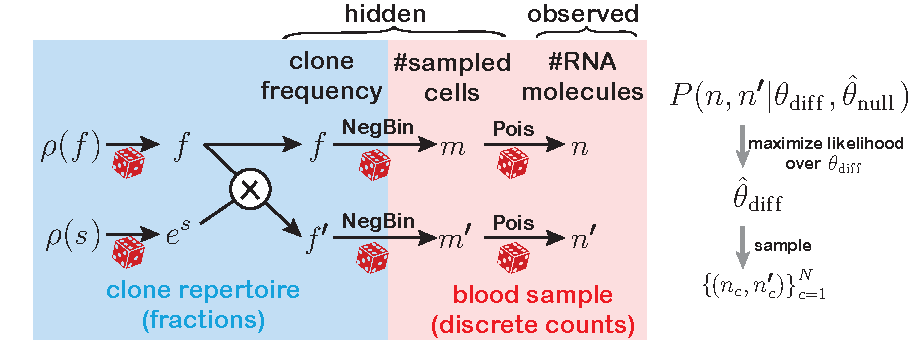
\includegraphics{fig2_diffexprmodel_schematic}
% \centering{}
% \caption{
% \emph{Differential expression model structure and learning procedure}. $P(n|f)$ is set as a negative binomial distribution in cell counts controlling the scale parameter of a Poisson distribution of molecule counts. In the differentially expressed condition (prime-decorated quantities), the parameters, $\theta_{diff}$, of the prior distribution, $\rho(c)$, of fold-change, $c$, are learned by maximizing the marginal likelihood (see section \textit{Fold change prior}) with respect to $\theta_{diff}$, keeping the remaining parameters, $\theta_{null}$, fixed to their ML estimates, $\hat{\theta}_{null}$, previously obtained using same-day replicate data (see fig. \ref{fig:nullstats}). 
% \label{fig:modelstruct}}
% \end{figure*}

% \begin{itemize}
% \item  A two-step, over-dispersed stochastic process most accurately captures the replicate statistics. 
% 
% \begin{itemize}
% \item  Single Pois fails qualitatively. see (Supp?) Fig. \ref{fig:suppfig1_Poisfail}.
% \item  Single NB and Pois->NB both outperformed in AIC/BIC by NB->Pois with model accuracy dominating over complexity (see Table \ref{Tbl1:NullModelCompare}). 
% \end{itemize}
% 
% \item Quality of best fit: See Fig. \ref{fig:modelfit}. The resulting model fits the data: not only the power law of the clone frequency distribution in the limit of large clones, but also the excess from that power law at small clone sizes due to finite sampling. It also captures the probability of pairs of counts that include a zero, i.e. that the clone was not identified in one of the samples. 
% %The model has no explicit dilution effect however, and so can not capture the overabundance of clones observed only once in the pair (i.e. where the other count is zero). (Show variance. fewer conditionals. How to show relative to Poisson? )
% 
% \item Sloppiness of parameter estimation: Show projections onto parameter axes of likelihood surface around maximum. Shows that $\gamma$ is tightly constrained. $a$ and $\delta$ tradeoff somewhat.
% \item Across day/donor variation: The natural variation models vary only systematically across days {\color{red} (check with rep size?)} , and do not depend strongly on the donor. We nevertheless use a donor-specific null model. Do time series of parameters, where result is that they are mostly flat. This would also show variability across donor.
% 
% \item Assess how well our model can fit the pre0-0 variation. Does it work? Why or why not.
% 
% \item Sampling self-consistency: Inference of sampled data is self-consistent: e.g. show over 10 random sampling of biorealistic range of values. See Fig. \ref{fig:suppfig2_reinf_null}.
% 
% \end{itemize}

% Text:
% We assume each clone has an intrinsic frequency,f, and we treat clones only by this frequency, not their sequence.
% We begin with a given rho(f), from which we sample a frequency which controls the mean and over-dispersion in the unobserved distribution of cells in the sample, which controls the mean number of a Poisson distribution of the observed number of RNA molecules. 
% We then sample the number of cells and molecules a second time for the second replicate and collect the result in the joint count distribution, P(n1,n2), which we fit to same day joint count histogram by adjusting the parameters of all previous steps, starting with the exponent of the power law.
% The joint count distribution is poorly sampled so I’ll instead show you how it fits the factored pieces:
% The conditional probability of observing some number of counts given that the other replicate had a given count, and we see that the bulk of the distributions shifts as we condition on higher values. 
% Next is the clone size distribution that inherits the power law of the hidden clone frequency distribution, though with some modifications that our model captures. 
% Finally, I wanted to show that the model even fits the data in cases when one of the two counts is zero. 
% I want to remind you that just because one count of an observed pair is 0, doesn’t mean it wasn’t in that repertoire, it just had a frequency that was too small for it to be picked up our sample. 
% Inferring the expansion from such small clones will be unreliable because they convey relatively little about what frequency produced them: It could have been anything below the detectable threshold, which is a wide range. 
% our method should reflect this.
% A single set of parameters is learned for each donor. Nevertheless, the learned null models are still specific to the day comparison to which they are applied because the value for the total number of cells for a replicate in the model is set by $m_T=N/r_c$, where $N$ is the total number of reads for that replicate.


% \begin{figure}[h!]
% %\includegraphics{procedure.png}
% \caption{
% \emph{Supp. Fig: Self-consistent reinference of null model}.
% \label{fig:suppfig2_reinf_null}}
% \end{figure}
% 
% \begin{figure}[h!]
% %\includegraphics{suppfig1_null_model_example}
% \caption{
% \emph{Supp. Fig: Failure with Poisson model}.
% \label{fig:suppfig1_Poisfail}}
% \end{figure}


\subsection*{Differential expression model}

\subsubsection*{model description}
Here, we use the null model to define and learn a model for differential expression. 
We set the clone frequency of the test condition as $f'=fe^s$, where $e^s$ is a multiplicative factor that we parametrize with a log-fold change, $s$. 
We incorporate $s$ as an additional random variable in the variable chain of the model by providing a prior on $s$, $\rho(s)$. 
$n$ and $n'$ are now conditionally independent given $f$ \textit{and} $s$.
As discussed in the Model Description section, the form of $\rho(s)$ depends on the application of the model. 
When used to describe a transient, selective perturbation relative to baseline, the form of $\rho(s)$ should contain a responding fraction with some effect size, alongside the non-responding component. 
The parameter values of these components can be chosen based on prior knowledge about typical sizes and fractions. 
Alternatively and best in the case of imprecise prior knowledge, $\rho(s)$ can be interpreted as part of the model and its parameter values learned directly from the data. 
Similar to the learning of the null model, here the corresponding marginal pair count distribution is 
\begin{equation}
    \begin{split}
	P(n,n'|\hat{\theta}_{\textrm{null}},\theta_{\textrm{diff}})=\iint P(n|f)P(n'|f'=fe^s)\rho(f)\rho(s)\text{d}s\text{d}f\;,
	\end{split}
\end{equation}
where we fix the null model parameters to their learned values, $\hat{\theta}_{\textrm{null}}$, and collect the parameters of $\rho(s)$ into $\theta_{\textrm{diff}}$. 
We satisfy the normalization constraint on $\vec{f'}$ by introducing into the given $\rho(s)$ an additional shift parameter, $s_0$, set to ensure, $Z^\mathcal{D}_{f'}=Z^\mathcal{D}_f$.
We then maximize this marginal likelihood over $\theta_{\textrm{diff}}$ to obtain the estimates. 

Constraints on cell population dynamics (e.g. division rates) suggest that the transformed frequencies in the differentially expressed condition should be bounded relative to those in the reference condition. 
In the absence of normalization, they can differ drastically, depending on the $\rho(s)$.
% Thus, as in the case of the null model where we added the normalization constraint on the sum of clone frequencies, here we must also impose some normalization on the sum of differentially expressed clones frequencies. 
% There are some families of $\rho(s)$, however, for which the ensemble average $\langle f'\rangle=\langle fe^s\rangle$ does not exist, e.g. all those not suppressing $e^s$ in the ensemble average over $s>0$ (Gaussian families being a notable exception). 
% Once we condition on a given realization, however, such averages remain finite. 
% To be independent of the form of $\rho(s)$ then, we normalize conditioned on a realized repertoire when sampling, and conditioned on observed data when inferring.
% While the normalization in the inference of the null model ensures that the ensemble average of $f$ is unity, even in the case of the differential expression model, the average over a realized repertoire can vary with the realization.
% A realization-specific normalization, instead of ensuring unit sum, ensures that the averages of the two frequencies be equal, $\langle f\rangle=\langle f'\rangle$. 


Once learned, the differential expression model provides for any observed clone the posterior distribution of log fold-change conditioned on the clone's observed count pair. 
It is calculated from the model by marginalizing $f$, and using Bayes' rule, 
\begin{align}
	P(s|n,n')=\frac{P(n,n'|s)\rho(s)}{P(n,n')}\;,
\end{align}
where $P(n,n'|s)=\int P(n|f)P(n'|f'=fe^s)\rho(f)\textrm{d}f\rho(s)$. 

\subsubsection*{Example 1: base prior and mouse repertoire}
To illustrate the behavior of the differential expression model, we present an application where
\begin{align}
	\rho_{s_0}(s)=\alpha\frac{1}{\bar{s}}e^{\frac{s_0-s}{\bar{s}}} \Theta(s-s_0)+(1-\alpha)\delta(s-s_0)\;, \label{eq:Ps_ex1}
\end{align} 
(see fig. \ref{fig:diffexpr_ex1}a). 
This choice describes a differentially expressed condition arising from a stimulus to which some fraction, $\alpha$, of the repertoire expands. 
Some of these clones respond strongly, most respond weakly, and all together with a characteristic effect size of log fold-change, $\bar{s}$, relative to non-responding clones in the remaining $1-\alpha$ fraction of the repertoire. 
$s_0>0$ shifts the probability mass to lower values of $s$. 
We set $s_0$ using the equal average frequency normalization constraint, ensuring that the sum of frequencies in the differentially expression condition equals that in the reference condition.
We inferred the parameters of the model from model-sampled synthetic $(n,n')$ data for both a small (mouse-like) and large (human-like \textcolor{red}{(still to do!)}) synthetic repertoire over a range of biologically plausible parameter values (see Methods for parameter values). 
In fig. \ref{fig:diffexpr_ex1}b, we show the inference problem of a mouse ($N=10^{6}$) repertoire for $(\bar{s}^*,\alpha^* )=(1.0,10^{-2})$, showing the errors are distributed optimally $\alpha$ and $\bar{s}$, i.e. they are given by the corresponding Fisher information, as expected from the fact that the MLE is efficient. To illustrate the structure of the posteriors computed from these learned models, in fig.\ref{fig:diffexpr_ex1}c, we show how the mass in the posteriors moves as we move in orthogonal directions in $(n,n')$ space. In particular, we see for example, that the width of the posterior narrows when counts are both large, and that the model ascribes no fold-change to clones with $n'< n$.

\begin{figure}[tbph!]
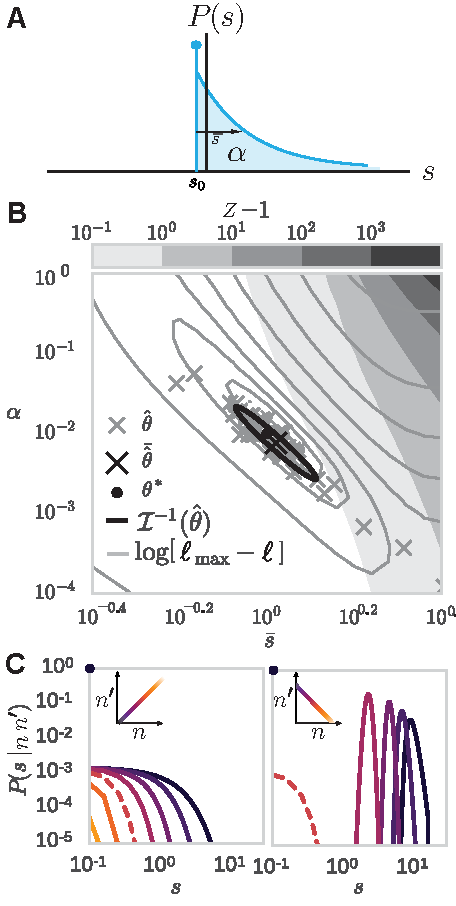
\includegraphics{fig5_diffexpr_eval}
\centering{}
\caption{
\emph{Inference on synthetic data.}(a) $\rho(s)$, eq. \ref{eq:Ps_ex1}, is parametrized by an effect size, $\bar{s}$, describing the expansion of the responding fraction, $\alpha$ of the repertoire. 
Expansion is relative to the functions center, $s_0$, which is fixed by the homeostatic constraint $\langle f \rangle=\langle f' \rangle$.
(b) Inferring $\theta^*=(\bar{s}^*,\alpha^* )=(1.0,10^{-2})$ (black dot). 
Maximums of the log-likelihood, $\ell_\textrm{max}=\ell(\hat{\theta}_r)$, for many realizations, $r=1,\dots,50$, are given by gray crosses, with their average, $\bar{\hat{\theta}}$, shown as the black cross. 
The log-likelihood, $\ell(\theta)$, for one realization is shown over logarithmically-spaced gray contours decreasing from the maximum, $\ell_{\textrm{max}}$. 
The inverse Fisher information, $\mathcal{I}^{-1}$, for a realization is shown as the black-lined ellipse centered around its maximum, $\bar{\hat{\theta}}$, provides a lower bound to the variance of our ML estimate. 
The gray scale contours increasing to the upper-right denote the excess in the used normalization, $Z=e^{s_0}$, above $1$. (c) Posteriors of the learned model, $P(s|n,n')$ over pairs $(n,n')$ for $n'=n$, with $n$ varying over a logarithmically-spaced set of counts (left), and for $n'$ given by the reverse order of this set (right). The black dot in both plots denotes the $1-\alpha$ non-responding component, $\delta(s-s_0)$.
(Parameters: $N=10^6$,$\epsilon=10^-2$.)
\label{fig:diffexpr_ex1}}
\end{figure}

\subsubsection*{Prior solvable via expectation maximization}
In the previous example, we performed a grid search followed by a quadratic approximation to obtain the maximum likelihood. In a more formal approach, here we employ expectation maximization (EM) to obtain the optimal parameter estimates from the data by calculating the expected log likelihood over the posterior and then maximizing with respect to the parameters. In practise, we perform the latter analytically and then evaluate the former numerically. We choose a symmetric exponential as a tractable prior for this purpose:
\begin{align}
	\rho_{\bar{s}}(s)=e^{-|s|/\bar{s}}/2\bar{s}
\end{align}
with $s\in\mathbb{R}$, $\bar{s}>0$. The expected value of the log likelihood function, often called the Q-function in EM literature, is 
 \begin{align}
 Q(\bar{s}|\bar{s}')=\sum_{(n,n')\in\mathcal{D}}^{N_\textrm{\textrm{obs}}}\int_{-\infty}^{\infty}\mathrm{d}s\rho(s|n,n',\bar{s}')\log \left[P(n,n',s|\bar{s})\right]\;,
 \end{align}
 where $\bar{s}'$ is the current estimate.
 Maximizing $Q$  with respect to $\bar{s}$ is relatively simple since $\bar{s}$ appears only in $\rho_{\bar{s}}(s)$  which is a factor in $P(n,n',s|\bar{s})$. For each $s$,
 \begin{align}
 \frac{\partial \log \left[\rho_{\bar{s}}(s))\right] }{\partial\bar{s}} &=\frac{1}{\rho_{\bar{s}}(s)} \frac{\partial\rho_{\bar{s}}(s)}{\partial\bar{s}}\\&=\frac{|s|-\bar{s}}{\bar{s}^2}\;,
 \end{align}
so that $  \frac{\partial Q(\bar{s}|\bar{s}')}{\partial\bar{s}}=\sum_{(n,n')\in\mathcal{D}}\int_{-\infty}^{\infty}\mathrm{d}s\rho(s|n,n',\bar{s}')\frac{\partial \log \left[\rho_{\bar{s}}(s))\right] }{\partial\bar{s}} =0$ implies
\begin{align}
  \sum_{(n,n')\in\mathcal{D}}\int_{-\infty}^{\infty}\mathrm{d}s\rho(s|n,n',\bar{s}')\frac{|s|-\bar{s}^*}{\bar{s}^{*2}} =0
\end{align}
so that $\bar{s}^*=\frac{1}{N_\textrm{\textrm{obs}}}\sum_{(n,n')\in\mathcal{D}}\bar{s}_{(n,n')}$, where 
\begin{align}
\bar{s}_{(n,n')}=\int_{-\infty}^{\infty}\mathrm{d}s|s|\rho(s|n,n',\bar{s}').
\end{align}
The latter integral is computed numerically from the model using $\rho(s|n,n',\bar{s}')=P(n,n',s|\bar{s}')/\int_{-\infty}^{\infty}P(n,n',s|\bar{s}')\mathrm{d}s	$. $Q$ is maximized at $\bar{s}=\bar{s}^*$ since  $ \frac{\partial^2 \log \left[\rho_{\bar{s}}(s))\right] }{\partial\bar{s}^2}\bigg|_{\bar{s}=\bar{s}^*}=-\bar{s}^{*-2} <0$. Thus, we update $\rho_{\bar{s}}(s)$ with 
\begin{align}
\rho_{\bar{s}}(s)\leftarrow\rho_{\bar{s}^*}(s).
\end{align}
The number of updates typically required for convergence was small.

\subsubsection*{Posteriors of log fold-change}

We can explain the shape of the posteriors by breaking up the model components into three groups: $P(n|f)\rho(f)$, which depends only on $f$, $\rho(s)$, which depends only on $s$, and the remainder depending on both $f$ and $s$, $P(n'|f'=fe^s)$. 
$P(n|f)\rho(f)$ contributes an exponential cutoff in $f$ near $n$.
$P(n'|f')$ contributes a similar cutoff in $f'$ near $n'$. 
$\log f$ and $s$ tradeoff in setting the value of $f'$.
Thus for fixed $s$, the cutoff in $f$ shifts to lower values for larger values of $s$.
For fixed $f$, the corresponding cutoff in $s$ shifts to larger values for smaller values of $f$, until a maximum cutoff in $s$ is reached for $f=f_\textrm{min}$.
This cutoff in $s$ can more strongly bound the posterior as we consider $(n,n')$ pairs with smaller $n/n'$.
However, this large $s$ cutoff can be gated by $\rho(s)$, depending on the form of its expansion ($s>0$) tail. 
In fact, the form of the decay of the expansion component of $\rho(s)$ interacts with the decay of $\rho(f)$. 
Indeed, for power law $\rho(f)$, $\log f$ is distributed exponentially, so that $\log f$ and $s$ tradeoff additively, not only in determining $f'$ but also in determining $\rho(f')$.
Which distribution, $\rho(f)$ or $\rho(s)$, dominates the shape of the posteriors then depends on the relative magnitude of their scale parameters.
\textcolor{red}{(Reader continues at their own peril)}.
\section{Rest is work in progress}
	
%An asymmetric exponential decay away from a shifted center at which a non-responding fraction is placed (see Eq. \ref{eq:genPs} and Fig. \ref{fig:Ps}).

% \begin{figure}[h!]
% \includegraphics{schematic}
% \centering{}
% \caption{
% \emph{Functional forms of prior on clone size log fold-change}. $\rho(s)$, eq. \ref{eq:genPs}, is parametrized most generally here by an effect size for both expansion, $s_+$, and contraction,$s_-$, with an expanded fraction, $\beta$ of changed clones, the latter fraction of which itself a parameter, $\alpha$. Expansion and contraction is relative to the functions center, $s_0$, which can be fixed by the constraint $\langle f_1 \rangle=\langle f_2 \rangle$.
% \label{fig:Ps}}
% \end{figure}


%\begin{table}%[H] add [H] placement to break table across pages
%\caption{Prior functions used. See Fig. \ref{fig:Ps} and Eq. \ref{eq:genPs}. $\langle f_1 \rangle= \langle f_2 \rangle$ adds constraint, e.g. fixes $s_0$. \label{Tbl1:Priors}}
%\begin{ruledtabular}
%\begin{tabular}{c|c|c|c|c|c|c|c}
%index	& label				&$\alpha$ & $\beta$	& $s_-$    	& $s_+$		& $s_0$  & \#DOF ($s_0$ fixed) \\
%\hline
%0 		& $flat$ shift 	 	&$\alpha$ & $1/2$  	& $\infty$	& $\infty$  & $s_0$  & 2 \\
%1 		& $L=R$ 	 		&$\alpha$ & $1/2$  	& $\bar{s}$	& $\bar{s}$ & $0$    & 2 \\
%2 		& $L=R$ shift		&$\alpha$ & $1/2$  	& $\bar{s}$	& $\bar{s}$ & $s_0$  & 3(-1) \\
%3 		& $R$ only   		&$\alpha$ & $0$    	& n/a       & $\bar{s}$ & $0$    & 2 \\
%4 		& $R$ only shift  	&$\alpha$ & $0$  	& n/a       & $\bar{s}$ & $s_0$  & 3(-1) \\
%5 		& $L\neq R$  		&$\alpha$ & $\beta$	& $s_-$    	& $s_+$     & $0$    & 4 \\
%6 		& $L\neq R$ shift  	&$\alpha$ & $\beta$	& $s_-$    	& $s_+$     & $s_0$  & 5(-1)
%\end{tabular}
%\end{ruledtabular}
%\end{table}

\begin{figure}[ht!]
%\includegraphics{procedure.png}
%centering{}
\caption{
\emph{Supp. Fig: Self-consistent reinference of diffexpr model}.
\label{fig:suppfig2_reinf_diffexpr}}
\end{figure}

\begin{figure}[ht!]
%\includegraphics{fig2_null_model_example}
%\centering{}
\caption{
\emph{Analysis of sloppiness of model: description of max-Likelihood manifold and possibly reduced description}
\label{fig:Data}}
\end{figure}

\begin{figure}[ht!]
%\includegraphics{fig2_null_model_example}
%\centering{}
\caption{
\emph{Evolution of parameters}. 
\label{fig:timeevo}}
\end{figure}

\begin{comment}
\begin{itemize}
  \item Supp fig: show self-consistent inference (See Fig. \ref{fig:suppfig2_reinf_diffexpr}).
  \item Explore space of fold-change priors (see Table \ref{Tbl1:Priors}) for representative 0-15 comparison (now just Azh, soon to be corroborated by results from all donors).
  \begin{itemize}
    \item  Prior 0: $\mathcal{L}^*=-4.2$, for $s^*_0\approx-3$, $\alpha^*=0$. At $s^*_0$, $\langle f_2\rangle/\langle f_1\rangle\approx10^{-3}.$
	\item  Prior 1: $\mathcal{L}^*=-1.952$, for $\bar{s}^*\to \infty $, $\alpha^*\to 0$: high plateau to left of edge ridge for $\alpha \propto \bar{s}^{-4}$
	\item  Prior 2: $\mathcal{L}^*=-1.96$. Same ridge, but with negative slope: $\bar{s}^*\to 0 $, $\alpha^*\to 1$.
	\item  Prior 3: Same as 2 for small $s_0$ and $\alpha$. slightly lower for larger values (-0.3). I.e. negative lobe has no effect for no shift.
	\item  Prior 4: Coming soon!
	\item  Prior 5: $\mathcal{L}^*=-1.953$, for $\bar{s}_+^*=1.0$, $\alpha^*=0.07$, $\bar{s}_-^*=0.86$, $\beta^*=0.11$ . small $\alpha$ is penalized (not so in prior 3,4).  %Similar to prior 2 except $\beta<1$ means that can get expanded right, independent of alpha, so that then too small alpha can be penalized. 
	\item  Prior 6: $\mathcal{L}^*=-1.954$, for $\bar{s}^*=0.67$, $\alpha^*=0.45$, $\bar{s}_-^*=0.9$, $\beta^*=0.11$. 
	\item  ...	still need to do free shift for Prior 1-6.
  \end{itemize}

  \item Using $\langle f_1\rangle=\langle f_2\rangle$ constraint to set $s_0$, gives $s^*_0<0$, which pulls down the likelihood at small $\alpha$, sculpting an interior maximum.

  \item Dynamics of ensemble parameters (See Fig. \ref{fig:timeevo}): 
  \begin{itemize}
	\item  the learned parameters, e.g. effect size and response fraction, give low response for same day (0-0, 0-pre0) comparisons.
	\item  Across days they grow and decay with the response. 
	\item  pre0 and 7 are similar to 0 (all compared to 0)?
	\item  pre0 is as different from 0 as day 7. 
  \end{itemize} 

  \item  Depending on legitimacy of pre0-0 null model, how does the prior parameter dynamics differ? are forward/backward distribution time-reversible?
\end{itemize}
\end{comment}
% (old) Text:
% 
% Armed with a well fit model of the same day variation, we generalized the model to apply to different days using a log fold change variable sampled from some distribution that controls the expansion or contraction that the second clone exhibits. 
% And, marginalizing out the hidden fold change variable, we again obtain a joint count distribution that we can use to fit the parameters of rho(s) to maximize the likelihood of the data. 
% We choose to restrict rho(s) to a two-parameter family of symmetric functions, with a parameter alpha the fraction of the repertoire that responds, and the sbar a typical effect size that controls the mean of a symmetric exponential function around 0 log fold change where the rest of clones are left as a delta function component.
% Doing the inference on alpha and sbar, and using the day 0 as the reference, we saw how the fraction of the perturbed repertoire rises and falls around day 15, as expected. 

\subsection*{Ensemble-level application: Time-tracking of ensemble parameters}

\subsection*{Clone-level application: Identification of responding clones}

Here we infer the posteriors from the learned differential expression model and show their utility by using them to obtain a list of significantly expanded clones as a result of yellow fever vaccination. 
\begin{figure}[ht!]
%\includegraphics{fig2_null_model_example}
%\centering{}
\caption{
\emph{Posteriors}. Some example posteriors. Distributions of slow, smed, shigh, and Pval. Volcano plot.
\label{fig:posteriors}}
\end{figure}


\begin{itemize}

\item  discuss posteriors and expansion probability over observed repertoire (Fig. \ref{fig:posteriors}): 
\begin{itemize}
	\item nature of (0,n) posteriors a result of balance of rho(f) and rho(s) priors.
	\item The distribution of posterior expansion probability shifts for different priors but maintains the rank of expansion across clones. 
\end{itemize}

\item  discuss significance tables.
\begin{itemize}
	\item  How much does the structure of the prior change the order and size of significance tables: e.g. shift/other parameters of prior correlates with size of list, i.e. location of cutoff.
	\item  ...
\end{itemize}

\item Is there any bias in the method?
\begin{itemize}
	\item  Sample from model and do ROC-like analysis showing quality of discrimination in tables. E.g. tends to underestimate large fold change. 
	\item ... 
\end{itemize} 

\end{itemize}


% Old Text from presentation:
% 
% To do that we look at the posterior probability of a clone being expanded or contracted for a given count pair, where here we plot it as a confidence and versus the pair’s expected fold change that comes out the model, a volcano plot, commonly used in RNAseq.
% We set a threshold on confidence and all pairs above this threshold are candidates for being selective to the vaccine. 
% Take a look at the two sets of points associated with the first count being 0 and 1, and with the second count of the data points increases with the expected fold change. 
% Remember that low counts convey little frequency and thus expansion information: the initial frequency could have been anything small and so we have to go to pretty high fold change, i.e. high n2, before we can say that this expansion is significant. 
% In particular, if we condition instead on the first count being 1, the expansion becomes significant at lower fold change, as the first count more reliably conveys information about it’s frequency. and so on with increasing count, and similarly for contraction.
% These are candidate clones ‘specific to the vaccines’. But how do we do we know that this is in fact the case.
% Experimental work performed a functional test by adding a gate for IFN gamma and sequenced this IFN enriched pool indeed show the vast majority show a strong functional response, validating our method. 


\section*{discussion}
\begin{itemize}
	\item  Procedure Summary:
		\begin{itemize}
			\item  used replicates to determine experimental clone size variability
			\item  inferred repertoire change distributions 
			\item  used to determine significantly expanded clones
			\item  validated using functional assay
		\end{itemize}
	\item  Natural variation results and discussion:
		\begin{itemize}
			\item  universal same-day variation. Implications...
			\item  Data tightly constrains power law frequency. Implications...
			\item  Nature of over-dispersion and order of NegBin/Pois.
		\end{itemize}
	\item  diffexpr results and discussion:
		\begin{itemize}
			\item  data strongly constrains prior expansion, not contraction. Implications...
			\item  Shift constraint and the relevance of homeostatis.

		\end{itemize}
    \item  application results and discussion:
		\begin{itemize}
			\item  posterior sensitivity to balance between $\gamma$ (prior for maximum expansion) and $\bar{s}$ (prior for characteristic expansion) in $(0,n)$ and $(n,0)$ pairs.
			\item  sensitivity of resulting tables. Note validation in Misha's paper.
			\item  Shift constraint and the relevance of homeostatis.
		\end{itemize}
	\item  Clinical use (reference Misha paper)
	\item  drawbacks of approach: need replicate data.
\end{itemize}


\section*{Methods}
%Our results are based on the posterior of differential fold change given an observed molecule count pair, which we infer directly from the data. Candidate responding clones were identified using a model of mRNA count statistics accounting for natural variation and differential expression and the sequencing process. Measured repertoires have a number of features that a model must capture to accurately reflect their statistics. First, for a clone to be observed it must appear in at least one of the pair of conditions, thus the support of the count distribution excludes $(n_1,n_2)=(0,0)$. While containing $10^6$ clones, these measured repertoires are still less than 1 percent of the full repertoire.

\subsection*{Null model definition}
The normalized clone size, $f$, is distributed according to the probability density function $\rho(f)$, bounded by $f_{\textrm{min}}\leq f \leq 1$, where $f_{\textrm{min}}^{-1}$ is an estimate of the total number of lymphocytes in an individual. Based on previous observations (Cite Weinstein 2009, Mora 2010, Mora 2016), $\rho(f)$ is set as a power-law, i.e. $\rho(f)\propto f^{-\gamma}$. We considered four different statistical models of cells and mRNA molecules contained in a sample. These used a negative binomial distribution, with parametrized over-dispersion: $\mathrm{NegBin}(\mu, \sigma^2=\mu+a \mu^{\beta})$ and a Poisson distribution, $\mathrm{Poisson}(\bar{s})$.

The final and highest scoring model is of cells sampled from a negative binomial and mRNA molecules from a Poisson distribution. A clone of size $f$ appears in a sample containing $M$ lymphocytes on average as $fM$ cells. To account for over-dispersed count statistics, the number of cells is set to be Negative-Binomial distributed with mean $fM$ and variance $fM+a (fM)^{\gamma}$, with $a>0$ the coefficient and $\gamma>1$ the power controlling the over-dispersion. For each clone, the number $n$ of detected mRNA molecules (i.e. UMI) is distributed according to a Poisson distribution with mean $mN_{\textrm{reads}}/M$, where $N_{\textrm{reads}}/M$ is the average number of UMI per cell, obtained using the observed total number of molecules, $N_{\textrm{reads}}$.
 
We inferred the parameters of this null model, $\theta_n=(\alpha,M,a,\gamma)$, from day-0 replicates by maximizing the likelihood of the observed count pairs, $(n,n')$, where $n\sim \mathrm{Poisson}(m N/M)$, $m\sim \mathrm{NegBin}(fM,fM+a (fM)^{\gamma})$, for each replicate, and $f\sim\rho$ is common to both replicates. For a given pair, the likelihood, $P(n,n'|\theta_{\textrm{null}})$, is obtained by marginalizing over $m,m'$, and $f$.

\subsection*{Normalization}
Here we derive the condition for which the normalization in the joint density is implicitly satisfied. The normalization constant of the joint density is
\begin{equation}
	\mathcal{Z}=\int_{f_\textrm{min}}^1\cdots\int_{f_\textrm{min}}^1\prod_{i=1}^N \rho(f_i)\delta(Z-1)\textrm{d}^N\vec{f} \;,
\end{equation}
with $\delta(Z-1)$ being the only factor preventing factorization and explicit normalization. Writing the delta function in its Fourier representation factorizes the single constraint on $\vec{f}$ into $N$ Lagrange multipliers, one for each $f_i$,
\begin{align}
	\delta(Z-1)&=\int_{-i\infty}^{i\infty} \frac{\textrm{d} \mu}{2 \pi}e^{\mu(Z-1)}  \\
	&=\int_{-i\infty}^{i\infty} \frac{\textrm{d} \mu}{2 \pi}e^{-\mu}\prod_{i=1}^N e^{\mu f_i} \;.
\end{align}
Crucially, the integral over $\vec{f}$ then factorizes. Exchanging the order of the integrations and omitting the clone subscript without loss of generality,
\begin{equation}
	\mathcal{Z}=\int_{-i\infty}^{i\infty} \frac{\textrm{d} \mu}{2 \pi} e^{-\mu} \prod_{i=1}^N \langle e^{\mu f}\rangle\;,\label{eq:bigZ}
\end{equation}
with $\langle e^{\mu f}\rangle=\int_{f_\textrm{min}}^1\rho(f)e^{\mu f}\textrm{d}f$. Now define the large deviation function, $I(\mu):=-\frac{\mu}{N}+\log \langle e^{\mu f}\rangle$, so that 
\begin{equation}
	\mathcal{Z}=\int_{-i\infty}^{i\infty} \frac{\textrm{d} \mu}{2 \pi} e^{-N I(\mu)}\;.\label{eq:largedev}
\end{equation}
Note that $I(0)=0$. With $N$ large, this integral is well-approximated by the integrand's value at its saddle point, located at $\mu^*$ satisfying $I'(\mu^*)=0$.  Evaluating the latter gives
\begin{align}
	\frac{1}{N}&=\frac{\langle f e^{\mu^* f}\rangle}{\langle e^{\mu^* f}\rangle}\;.
\end{align} 
If the left-hand side is equal to $\langle f\rangle$, the equality holds only for $\mu^*=0$ since expectations of products of correlated random variables are not generally products of their expectations. 
In this case, we see from eq.\ref{eq:largedev} that $\mathcal{Z}=1$, and so the constraint $N\langle f\rangle=1$ imposes normalization.
% \begin{align}
% 	\langle g(\vec{f})\rangle_{\rho_N(\vec{f})}&=\int_{f_\textrm{min}}^1\cdots\int_{f_\textrm{min}}^1\prod_{i=1}^N \rho(f)\frac{1}{2 \pi} \int_{-i\infty}^{i\infty} e^{i \mu(Z-1)} \textrm{d} \mu \textrm{d}^N\vec{f} g(\vec{f})\\
% 	\int_{f_\textrm{min}}^1\cdots\int_{f_\textrm{min}}^1\prod_{i=1}^N \rho(f)\frac{1}{2 \pi} \int_{-i\infty}^{i\infty} e^{i \mu(Z-1)} \textrm{d} \mu \textrm{d}^N\vec{f} g(\vec{f})\;.
% \end{align}
\subsection*{Obtaining diversity estimates from the clone frequency density}
For a set of clone frequencies, $\{f_c\}_{c=1}^{N}$, for a set of clones, the Hill family of diversities are obtained from the Renyi entropies, as $D_\beta=\exp H_\beta$, with $H_\beta=\frac{1}{1-\beta}\ln \left[ \sum_c f_c^{\beta}\right]$. We use $\rho(f)$ to compute their ensemble averages over $f$, again under the assumption that the joint distribution of frequencies factorizes. We obtain an estimate for $D_0=N$ using the model-derived expression, $N_{1,samp}+P(n=0)N=N$, where $N_{1,samp}$ is the number of clones observed in one sample, and $P(n=0)=\int_{f_{\textrm{min}}}^1 P(n=0|f)\rho(f)\textrm{d}f$. For $\beta=1$, we compute $\exp (N\langle -f\log f \rangle_{\rho(f)})$ and for $\beta=2$, we use $1/\left(N\langle f^2\rangle_{\rho(f)}\right)$.

\subsection*{Null Model Sampling}
The procedure for null model sampling is summarized as (1) fix main model parameters, (2) solve for remaining parameters using the normalization constraint, and (3) starting with frequencies, sample and use to specify distribution of next random variable in the chain.

In detail, we first fix:
\begin{itemize}
\item  the model parameters $(\alpha,M,a,\gamma)$, excluding $f_{\textrm{min}}$. Separate $M$, $a$, and $\gamma$ values could be defined for the reference and test condition, respectively. The empirical $P(n,n')$ for replicate data was found to be highly symmetric in $n$ and $n'$ across donors, however, supporting the assumption of a single acquisition model and so we neglect this complication. 
\item  the desired size of the full repertoire, $N$. 
%Together with the model prediction of capture efficiency, $1-P(0,0)$, this gives the number of clones we should sample, $N_{\textrm{\textrm{obs}}}$, via $N_{\textrm{\textrm{obs}}}=N(1-P(0,0))$, 
\item the sequencing efficiency (total sample reads/total sample cells), $\epsilon$. From this we get the effective total sample reads, $N_{\textrm{reads}}=\epsilon M$, that converts a clone's frequency to the average number of cells it appears with in the sample. (We could in fact define two sequencing efficiencies, one for each replicate, leading to different effective total number of reads in each replicate). Note that the actual sampled number of reads is stochastic and so will differ from this fixed value.
\end{itemize}
We then solve for remaining parameters. Specifically, $f_{\textrm{min}}$ is fixed by the constraint that the average sum of all frequencies, under the assumption that their distribution factorizes, is unity:
\begin{equation}
% 	P(0,0)N\langle f\rangle_{\rho(f|n+n'=0)} + N_{\textrm{\textrm{obs}}} \langle f\rangle_{\rho(f|n+n'>0)} = 1
	N \langle f\rangle_{\rho(f)}=1
\end{equation}
This completes the parameter specification.

We then sample from the corresponding chain of random variables.
Sampling the chain of random variables of the null model can be performed efficiently by only sampling the $N_{\textrm{obs}}=N(1-P(0,0))$ observed clones. This is done separately for each replicate, once conditioned on whether or not the other count is zero (see appendix for this procedure). Here, we instead perform the inefficient but more straightforward procedure of sampling all $N$ clones and discarding those clones for which $(n,n')=(0,0)$. A slight difference in the two procedures is that $N_{\textrm{obs}}$ is fixed in the former, while is stochastic in the latter.

Using this sampling procedure we demonstrate the validity of the null model and its inference by sampling across the observed range of parameters and reinferring their values (See fig. \ref{fig:reinfer_null}).

\subsection*{Null Model Inference}
Given a data set, $\mathcal{D}=\{(n_i,n'_i)\}_{i=1}^{N_{\textrm{obs}}}$, we infer the parameters of the null model, $\Theta_{\textrm{null}}=(\alpha,a,\gamma,M,f_{\textrm{min}})$ by maximizing the marginal likelihood of the observable model, $P(n,n'|n+n'>0,\Theta_{\textrm{null}})$, subject to the normalization constraint$, N\langle f\rangle_{\rho(f)}=1$, where $N=N_{\textrm{obs}}/(1-P(0,0))$. Since in this case we have access to a realization, we could instead normalize conditioned on this realization. Since, 
\begin{equation*}
	N\sum_{(n,n')>0}P(n,n')\approx N\sum_{(n,n')\in \mathcal{D}}\frac{\#(n,n')}{N}\equiv \sum_{i}^{N_{\textrm{obs}}}
\end{equation*}
we then have
\begin{equation}
	1=N\langle f\rangle_{\rho(f|\mathcal{D})}
							   = P(0,0)N\langle f\rangle_{\rho(f|n+n'=0)} + \sum_{i}^{N_{\textrm{obs}}}\langle f\rangle_{\rho(f|n_i,n'_i)}\;.
\end{equation}

\subsection*{Differential expression model definition}
We introduce a selection factor $s$ defined as the log-fold change between a clone's frequency on one day, $f$, and that on another, $fe^s$, and define $P(n_1,n_2|s,\theta_n)$ as before, but replacing $f$ by $fe^s$ in the definition of $m_2$. Given a prior distribution  $P(s|\theta_s)$ over $s$ parametrized by a set of parameters $\theta_s$ distinct from $\theta_n$, we used Bayes rule to obtain the posterior log fold-change probability function given an observed count pair, $P(s|n_1,n_2,\theta_n,\theta_s)$. We set the values of the parameters $\theta_s$ of this prior by again maximizing the likelihood of the count pair data given the model over $\theta_s$, $\int P(n_1,n_2|s,\theta_n)P(s|\theta_s)\textrm{d}s$.

We explored a family of priors expressible as 
\begin{eqnarray}
	P(s|\theta_s)&=&\frac{\alpha \beta}{Z_+}e^{-\frac{|s-s_0|}{s_+}}\Theta(s-s_0) \nonumber\\
	&&+\frac{\alpha (1-\beta)}{Z_-}e^{-\frac{|s-s_0|}{s_-}}\Theta(s_0-s) \\
	&&+(1-\alpha)\delta(s-s_0)\;, \label{eq:genPs}\nonumber
\end{eqnarray}
with $Z_{\pm} \sim s_{\pm}$ (see Fig. \ref{fig:Ps}) so that in the most general prior, $\theta_s=(s_-,s_+,\alpha,\beta,s_0)$. See table \ref{Tbl1:Priors} for reduced-parameter versions of this model that we considered.

\subsection*{Identifying responding clones}
In analogy with $p$-values, we used the posterior probability corresponding to the null hypothesis that they are not expanded, $p=P(s\leq s_{thr}|n_1,n_2,\theta_n,\theta_s)$ to rank the clones by the significance of their expansion, using a threshold of $p<0.025$ and a threshold effect size of $s_{thr}$. 

\begin{figure}[ht!]
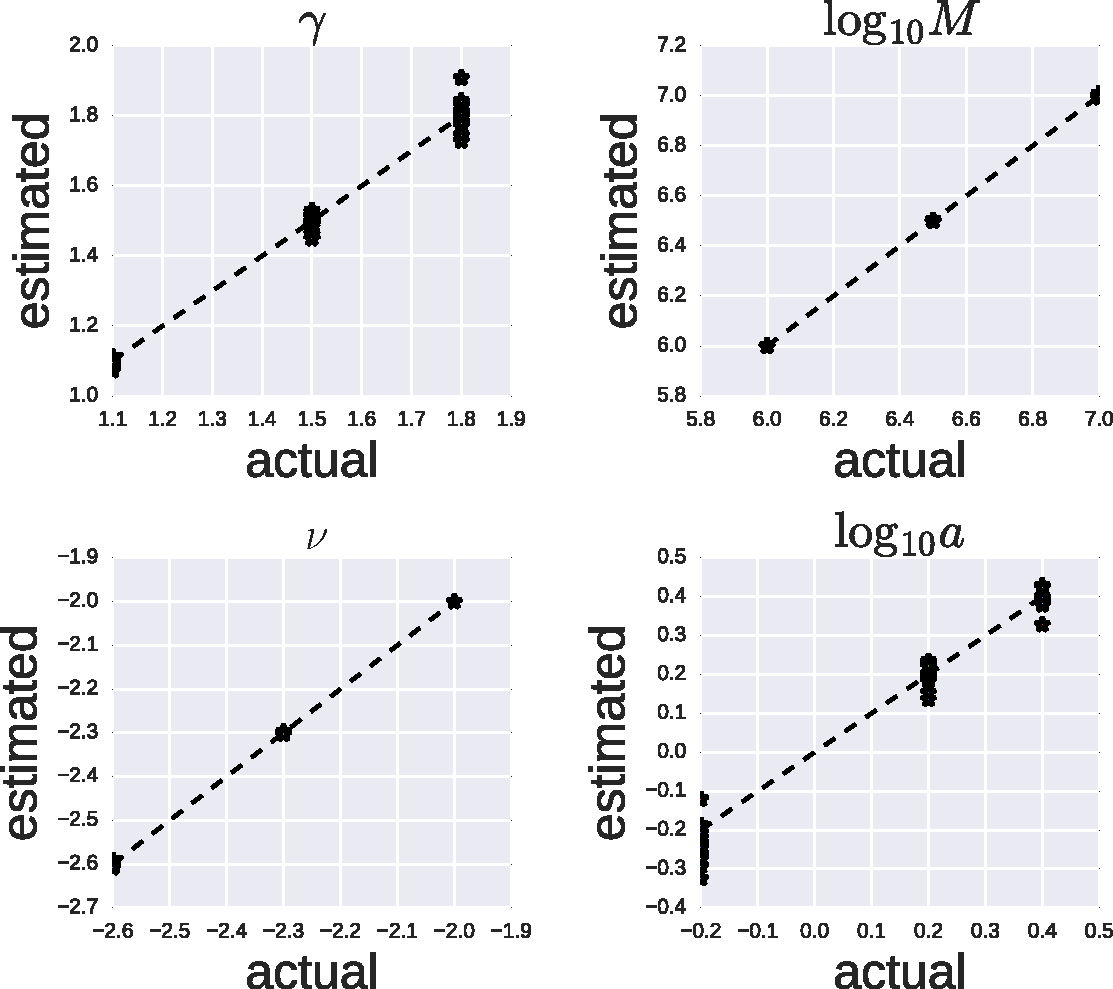
\includegraphics[width=\linewidth]{NB_Pois_nullpara_fits}
\centering{}
\caption{
\emph{Reinferring null model parameters}. Shown are the actual and estimated values of the null model parameters used to validate the null model inference procedure over the range exhibited by the data. A 3x3x3x3 grid of points were sampled and results collapsed over each parameter axis. $f_{min}$ was fixed to satisfy the normalization constraint.
\label{fig:reinfer_null}}
\end{figure}

\subsection*{Alternative model sampling procedure}
Since the differential expression model involves expansion and contraction in the test condition, some normalization in this condition is needed such that it produces roughly the same total number of cells as those in the reference condition, consistent with the observed data. One approach (the one taken below) is to normalize at the level of clone frequencies. 

\subsubsection*{Direct Sampling}
The frequencies of the first condition, $f_i$, are sampled from $\rho(f)$ until they sum to 1 (i.e. until before they surpass 1, with a final frequency added that takes the sum exactly to 1). An equal number of log-fold changes, $s_i$, are sampled from $\rho(s)$. The normalized frequencies of the second condition are then $f'_i=f_ie^{s_i}/\sum_j f_je^{s_j}$.  Counts from the two conditions are then sampled from $P(n|f)$ and $P(n'|f')$, respectively. As a final step, unobserved clones, i.e. those with $(n,n')=(0,0)$, are discarded.

\subsubsection*{Effective Sampling}
For an efficient implementation, the procedure should avoid sampling the numerous clones that produce $(n,n')=(0,0)$, since these are discarded. Such a procedure follows. 

First, the $(f,s)$-plane is partitioned into two regions, $D=\{(f,s)|f<f_0,fe^s<f_0\}$ and its complement, $\bar D$, with $f_0$ chosen such that clones sampled from $\bar D$ are often \textit{observed}, i.e. $n+n'>0$ (a minority of clones sampled in $\bar D$ will nevertheless give $n+n'=0$; these are discarded). In contrast, frequencies sampled from $D$ will be small, so that most will be unobserved, and we must condition on the clone being observed when sampling from this regime. Moreover, their average is unaffected by the long-tailed behaviour of the distribution in the large-frequency regime and thus is well-approximated by the corresponding ensemble average. We use this latter fact when computing the renormalization of the frequencies of the second condition. 

We compute the mass in $D$ as $P_D=\int_f \textrm{d}f\rho(f)\sum_s \rho(s) \mathbb{1}((f,s)\in D)$.

We sample $(f,s)$ in $\bar D$ until the sum of the first condition's frequencies, $\sum_i f_i$ added to the expected sum in $D$, $P_D N_{cl}\langle f\rangle_{P(f|D)}$, equals 1,
\begin{align}
	1=\sum_{i=1}^{N_{\bar D}} f_i + P_D N_{cl}\langle f\rangle_{P(f|D)}\;,
\end{align}
where $N_{cl}$ is the total number of clones in the repertoire. The number sampled from $\bar D$, $N_{\bar D}$, is determined from that expression self-consistently by substituting $N_{cl}=N_{\bar D}/(1-P_D)$ obtained from $N_{\bar D}+P_D N_{cl}\equiv N_{cl}$. The normalization for the second condition's frequencies is then 
\begin{align}
	Z=\sum_{i=1}^{N_{\bar D}} f_ie^{s_i} + P_D N_{cl}\langle fe^s\rangle_{P(f,s|D)}
\end{align}
such that the second condition's frequencies are ${f_i'=f_ie^{s_i}/Z}$. Molecule counts are then sampled from $P(n|f)$ and $P(n'|f')$.  

We then sample from $D$ conditioned on the clone being observed, i.e. having produced a finite number of molecules in either of the two conditions. We thus sample $N_D=P(n+n'>0|D)P_D N_{cl}$ clones from $P(f,s|D,n+n'>0)$. To avoid having to sample over the joint distribution of $n$ and $n'$, we condition on the 3 regions of finite counts in both conditions, $(n,0)$, $(0,n')$, and $(n,n')$, in which $n$ and $n'$ can be sampled independently. 
Note the presence of the normalization factor, $Z$, in 
\begin{align}
	P(n+n'>0|D)=\int_f \textrm{d}f\rho(f)\sum_s \rho(s)(1-P(n=0|f)P(n'=0|f'=fe^s/Z))\;.
\end{align}
and
\begin{align}
	P(f,s|D,n+n'>0)=\frac{\rho(f)\rho(s)(1-P(n=0|f)P(n'=0|f'=fe^s/Z))}{P(n+n'>0|D)P_D}\;.
\end{align}
We then concatenate the $N_D$ sampled counts from $D$ and the $N_{\bar D}$ sampled counts (with $(n,n')=(0,0)$ realizations discarded) from $\bar D$ to obtain the full data set.  

\subsection*{equal frequency constraint}
The constraint of equal frequencies in the two compared conditions, $\langle f_1\rangle=\langle f_2\rangle$ can be satisfied with a suitable choice of the shift parameter, $s_0$, in the prior for differential expression, $\rho(s)$. The ensemble average can be evaluated over $p(f,s|n_1+n_2>0)$, where $f_1=f$ and $f_2=f e^s$, where 
\begin{align}
	P(f,s|n_1+n_2>0)&=&\frac{\sum_{n_1+n_2>0}{P(n_1,n_2,f,s)}}{\sum_{n_1+n_2>0}\int{\textrm{d}f \sum_s P(n_1,n_2,f,s)}} \\
					&=&\frac{\sum_{n_1+n_2>0}{P(n_1,n_2,f,s)}}{\sum_{n_1+n_2>0}\int{\textrm{d}f \sum_s P(n_1,n_2,f,s)}}
\end{align}
and using this, $P(f|n_1+n_2>0)=\sum_s P(f,s|n_1+n_2>0)$. The shift enters in $P(n_1,n_2,f,s)=P(n_1|f)P(n_2|f,s)P(f)P_{s_0}(s)$ via $P_{s_0}(s)$. A convenient change of variables $s\leftarrow\Delta s+s_0$ maps $P_{s_0}(s)$ to $P_{0}(\Delta s)$, upon which
\begin{align}
	\langle fe^s \rangle &=&\int{ \textrm{d}f \sum_{\Delta s} fe^{\Delta s+s_0} P(n_1|f)P(n_2|f,\Delta s+s_0)P(f)P_{0}(\Delta s)} \\
						 &=&e^{s_0}\int{ \textrm{d}f \sum_{\Delta s} fe^{\Delta s} P(n_1|f)P(n_2|f,\Delta s+s_0)P(f)P_{0}(\Delta s)}
\end{align}
denoting the remaining integral, $\tilde{\langle fe^s \rangle}$, and performing the same change of variables on $\langle f \rangle$,
\begin{align}
	\langle f \rangle &=&\int{ \textrm{d}f \sum_{\Delta s} f             P(n_1|f)P(n_2|f,\Delta s+s_0)P(f)P_{0}(\Delta s)}\;,
\end{align}
and so the condition can be written as $s_0=\ln \tilde{\langle fe^s \rangle} - \ln \langle f \rangle$. To obtain $s_0$ from this implicit equation, we apply an iterative scheme beginning with $s_0=0$. We compute $P(n_2|f,\Delta s+s_0)$, and then the latter expression supplies $s_0$ in the next iteration. In practice, we take a bounded range of $\Delta s$ symmetric around 0. Thus, the only factor containing shift information is $P(n_2|f,\Delta s+s_0)$ appearing in both $\tilde{\langle fe^s \rangle}$ and $\langle f \rangle$. However, for correspondence with numerics, the $e^{\Delta s}$ factor must be defined over a shifted domain.

Alternatively, the average can be computed over the data directly, via $\langle fe^s \rangle=\frac{1}{N_{pairs}}\sum_{(n_1,n_2)}\langle fe^s \rangle_{P(f,s|n_1,n_2)}$. The should converge to the analytical result in the limit of many clones (and some other condition?).
%\lange fe^s \rangle &=&\int{ \textrm{d}f \sum_s fe^s p(f|n_1+n_2>0)}\;,

% Candidate responding clones were identified using a model of RNA count statistics accounting for differential expression and the sequencing process. A full presentation will be published elsewhere. Here, we provide a brief exposition of the model and how we have applied it. The core repertoire object in the model is a probability density function, $\rho(f)$, of normalized clone size, called clone frequency, $f\in[1/m_{total},1]$, where $m_{total}=10^{11}$ is an estimate of the total number of lymphocytes in an individual. $\rho(f)\mathrm{d}f$ is then the probability that a randomly sampled clone takes up a fraction $f$ of the repertoire. We set $\rho(f)\propto f^{\gamma}$, i.e. power-law distributed with the power $\gamma<0$, consistent with many observed unpartitioned sampled repertoires.
% 
% Next, a blood sample contains a sampled repertoire in the form of an a priori unknown number of lymphocytes, $m_{sample}$. Across many clones of size $f$ in the sample, these will appear on average with $\bar{m}(f)=fm_{sample}$ cells. In our data and elsewhere, prevalent overdispersion is observed in the count statistics. We thus employ the mean-variance relation, $\sigma_m^2(f)=\bar{m}(f)+a \bar{m}(f)^{\beta}$, with $a>0$ the coefficient and $\beta>1$ the power controlling the over-dispersion. We set the number of cells to be Negative-Binomial distributed with mean $\bar{m}(f)$ and variance $\sigma_m^2$. 
% 
% Finally, the cells in the sample are then barcode-sequenced, resulting in a number of putative RNA molecules, $n$, for each clone. $m$ cells will produce $\bar{n}(m)=mr_c$ molecules on average where $r_c>0$ is the average number of RNA molecules per cell. $r_c$ brings together into a single parameter a variety of diluting effects, heterogeneous across samples so that we expect $r_c<1$. For an total observed number of observed reads, $n_{sample}$, $r_c$ is related to $m_{sample}$ via $n_{sample}=r_cm_{sample}$. Even though $m_{sample}$ is precisely controlled by the sampled volume, $n_{sample}$ still varies due to procedural variation in sequencing. Thus, we let $r_c$ account for this variation by setting it as $r_c=m_{sample}/n_{sample}$. We set the number of molecules to be Poisson-distributed with scale parameter $\bar{n}(f)$.
% 
% We used day-0 replicates to infer maximum likelihood estimates for these parameters using the likelihood function,
% \begin{align}
% \mathcal{L}(\gamma,m_{sample},a,\beta)=\frac{1}{N_{clones}}\sum_{(n_1,n_2)_{data}}\log P_{\mathrm{same}}(n_1,n_2)
% \end{align}
% where $N_{clones}$ is the number of observed clones and
% \begin{align}
% P_{\mathrm{same}}(n_1,n_2)&=\int_{1/m_{total}}^1P(n_1|f_1=f)P(n_2|f_2=f)\rho(f)\mathrm{d}f\\
% P(n|f)&=\sum_{m=0}^{\infty}\mathcal{NB}_{\bar{m}(f),\sigma^2_{m}(f)}(m)Pois_{\bar{n}(m)}(n)\;.
% \end{align}
% This fitted model characterizes the variation expected of pairs of sampled repertoires for unchanged antigen conditions.
% 
% For changing antigen conditions, the clone frequencies making up the repertoire will change. Using $s$ to denote the log-fold change between a clone's frequency in one condition, $f_1$, and another $f_2=f_1e^s$, a distribution of these changes, $\rho(s)$, exists. A particular $\rho(s)$ serves as a prior distribution for these changes. The posterior probability given an observed count pair is then
% \begin{align}
% P(s|n_1,n_2)\propto P(n_1,n_2|s)\rho(s)
% \end{align}
% where 
% \begin{align}
% P(n_1,n_2|s)=\int_{1/m_{total}}^1P(n_1|f_1=f)P(n_2|f_2=fe^s)\rho(f)\mathrm{d}f\;.
% \end{align}
% Note the additional factor of $e^s$ compared with the same-day model in the expression for $f_2$. 
% The posterior distribution of fold change given an observed count pair can be used to rank the clones by the significance of their expansion. In analogy with p-values, we use the posterior probability corresponding to the null hypothesis that they are not expanded, $P(s\leq 0|n_1,n_2)$ and set a threshold of significance $P(s\leq 0|n_1,n_2)\leq 0.025$. 
% 
% We parametrize our prior, $\rho(s)$, with  $\alpha\in[0,1]$, the fraction of clones that responds to the change, and $\bar{s}>0$, their typical effect size. Accordingly, we set $\rho(s)=\frac{\alpha}{Z}\exp\left[-|s|/\bar{s}\right]+(1-\alpha)\delta(s)$, where the normalization, $Z$, is such that the first term integrates to $\alpha$. We set the values of the parameters of this prior by again maximizing the likelihood of the data given the corresponding model,
% \begin{align}
% \mathcal{L}(\alpha,\bar{s})=\frac{1}{N_{clones}}\sum_{(n_1,n_2)_{data}}\log P_{\mathrm{diff}}(n_1,n_2)
% \end{align}
% where
% \begin{align}
% P_{\mathrm{diff}}(n_1,n_2)=\int_{s_{min}}^{s_{max}}P(n_1,n_2|s)\rho(s)\mathrm{d}s\;.
% \end{align}

\section*{Acknowledgements}
...would like to acknowledge discussions with ... This work was supported by ... 

\section*{Author Contributions}
M.P.T., A.W., T.M. ... 

\section*{Additional Information}
The authors declare no competing financial interests.

\appendix
\section{Appendixes}
Samples with 0 molecule counts can in principle be produced with any number of cells, so cell counts must be marginalized when implementing this constraint. We thus used the conditional probability distributions $P(n_i|f)=\sum_{m_i}P(n_i|m_i)P(m_i|f)$ with $m_i,m_i,n_i,n_i=0,1,\dots$ and $i=1,2$. Note that these two conditional distributions differ only in their average number of UMI per cell, $N_i/M$, due to their differing the observed total number of molecules, $N_i$. Together with $\rho(f)$, these distributions form the full joint distribution, which is conditioned on the clone appearing in the sample, i.e. $n_1+n_2>0$ which we denote $C$ for clarity, 
\begin{align}
	P(n_1,n_2,f|C)= \frac{P(n_1|f)P(n_2|f)\rho(f)}{1-\int{\textrm{d}f \rho(f)\textrm{d}f P(n_1=0|f)P(n_2=0|f)}}\;,  
\end{align}
with the renormalization accounting for the fact that $(n_1,n_2)=(0,0)$ is excluded. The 3 quadrants having a finite count for at least one replicate are denoted $q_{x0}$, $q_{0x}$, and $q_{xx}$, respectively. Their respective weights are
\begin{align}
	P(q_{x0}|C)&=&\sum_{n_1>0}\int{\textrm{d}f P(n_1,n_2=0,f|C)}\;,\\
	P(q_{0x}|C)&=&\sum_{n_2>0}\int{\textrm{d}f P(n_1=0,n_2,f|C)}\;,\\
	P(q_{xx}|C)&=&\sum_{\substack{n_1>0,\\n_2>0}}\int{\textrm{d}f P(n_1,n_2,f|C)}.
\end{align}
Conditioning on $C$ ensures normalization, $P(q_{x0}|C)+P(q_{0x}|C)+P(q_{xx}|C)=1$. Each sampled clone falls in one the three regions according to these probabilities. Their clone frequencies are then drawn conditioned on the respective region, 
\begin{align}
	P(f|q_{x0})&=&\sum_{n_1>0}P(n_1,n_2=0,f|C)/P(q_{x0}|C)\;,\\
	P(f|q_{0x})&=&\sum_{n_2>0}P(n_1=0,n_2,f|C)/P(q_{0x}|C)\;,\\
	P(f|q_{xx})&=&\sum_{\substack{n_1>0,\\n_2>0}}P(n_1,n_2,f|C)/P(q_{xx}|C).
\end{align}
Using the sampled frequency, a pair of number of cells $(m_1,m_2)$ is obtained. For $q_{x0}$, $m_1$ is sampled from $P(m_1|f,n_1>0)$ and $m_2$ sampled from $P(m_2|f,n_2=0)$ with 
\begin{align}
	P(m_1|f,n_1>0)&=&\frac{\sum_{n_1>0}P(m_1,n_1|f)}{\sum_{\substack{n_1>0,\\m_1}}P(m_1,n_1|f)}\;,\\
	P(m_2|f,n_2=0)&=&\frac{P(m_2,n_2=0|f)}{\sum_{m_2}P(m_2,n_2=0|f)}\;,
\end{align}
with $P(m_i,n_i|f)=P(n_i|m_i)P(m_i|f)$, for $i=1,2$. Note that by construction here, $m_1>0$, since $P(n_1>0|m_1=0)=0$.
The procedure is similar for frequencies sampled in $q_{0x}$. For frequencies sampled in $q_{xx}$, cell count pairs $(m_1,m_2)$ are sampled from $P(m_1|f,n_1>0)$ and $P(m_2|f,n_2>0)$, respectively. 

Molecule counts for the three quadrants are then sampled as $(n_1,0)$, $(0,n_2)$, and $(n_1,n_2)$, respectively, with $n_1$ and $n_2$ drawn from the renormalized, finite-count domain of the conditional distributions, $P(n_1|m_1)$ and $P(n_2|m_2)$, respectively, with $m_1>0$ and $m_2>0$. 

\bibliography{diffexpr}

\end{document}  












